\section{Combining Storage Systems with COMPSs}
\label{sec:storage}
Most COMPSs objects are created by the user and managed by the Runtime. The data transferring software is a self-made library based on NIO \footnote{https://docs.oracle.com/javase/7/docs/api/java/nio/package-summary.html}. Although this is usually a good enough solution for most use cases, there are three scenarios in which it may be a disadvantage to use this library:

\begin{enumerate}
\item The objects are the output of some previous application
\item The outputs of the COMPSs application are the input of some other application
\item The filesystem and/or the network presents huge bandwidth limitations
\end{enumerate}

The two first items represent a common usability problem. Many research groups generate their inputs 
%TODO: FINISH THIS CHAPTER

\subsection{Defining a Storage API}
\label{subsec:storage_api}
The need of defining a storage API comes from the fact that some researchs groups are interested into mixing some of their tools with the COMPSs Programming Model. After some meetings with these groups it was decided 
%TODO: ALSO FINISH THIS ONE

\subsection{A Practical Implementation: Redis}
\label{subsec:storage_redis}
The first step towards validating this storage API consisted of providing a valid, functional implementation. For this purpose Redis was chosen.\\
\\
Redis \footnote{https://redis.io/} is a simple Key-Value distributed storage database. Redis can be seen as a distributed hash map with $2^14 = 16384$ slots. Each key is either chosen by the user or randomly assigned, and it determines the position of this object in the hash table. More precisely, given a key $k$, and a value $v$, $v$ will be stored at the position $\textrm{CRC16}(k) \mod \quad 16384$. CRC16\footnote{https://en.wikipedia.org/wiki/Cyclic\_redundancy\_check} is a known checksum-like method used by many devices and network protocols to check that a message has been sent with no errors, and it can also be used as a quick hash function.\\
\\
Our implementation serializes objects in-memory and stores them as byte arrays in the database. Although this does not save us from serializing objects it is enough to avoid dealing with the filesystem, and to do all the operations in-memory. Huge byte arrays are split in distributed blocks to avoid long-term load imbalances and to increase long-term data locality. If we have $N$ worker nodes, our data is $M$ bytes long, it is available at only one node, and nodes are busy enough to make data locality irrelevant then the expected data transferring time is
$$E_1[N] = \frac{N - 1}{N} \times M$$
If our data is split into $K$ blocks, $\frac{M}{K}$ bytes each block, and each block is at a different node then the expected data transferring time can expressed as

$$E_2[N] \leq \frac{K}{N}(K - 1)\frac{M}{K} + \frac{N - K}{N}M$$

By simplifying $M = 1$ we obtain that $E_2[N] \leq E_1[N] = \frac{N - 1}{N}$. However, this second approach offers the opportunity to introduce parallelism and, in fact, most practical applications show that the required time to transfer the $(K - 1)$ remaining blocks is usually less or equal than $2.5\frac{M}{K}$, or something around that, and that in the worst case scenario the introduced overhead is relatively negligible, which is consistent with the two formulas above.

Another detail about our Redis implementation is that Redis offers no direct way to make some piece of data end in some node. However, the Storage API defines a method which allows the user to do that. Our solution to this problem consisted of simply generating random keys until one of them mapped to a valid slot. This adds almost no overhead, as the number of nodes tends to be a very manageable number such as 16, 32, 64, or at most 128 in most practical cases.

\subsection{Practical Applications}
\label{subsec:storage_apps}
\subsubsection{K-Means}
\label{subsubsec:kmeans_redis}
K-Means \cite{Lloyd82leastsquares} is a clustering algorithm which, given $N$ $k$-dimensional points and an integer $c$, assigns each point a label between $1$ and $c$. The idea is that these labels represent groups of \textit{similar} points. An example of what this algorithm computes can be found in figure \ref{fig:kmeans_example}.

\begin{figure}
\centering
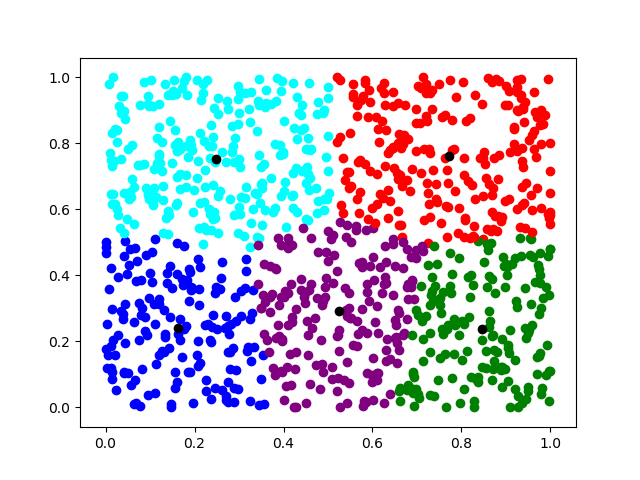
\includegraphics[scale = 0.5]{figures/kmeans_example.png}
\caption{A set of points grouped by the K-Means algorithm. Black points represent centroids, colours represent different groups}
\label{fig:kmeans_example}
\end{figure}

The algorithm can be sumarized as follows:

\begin{enumerate}
\item Generate $c$ random $d$ dimensional points, call them \textit{centroids}
\item For each point of the input data, compute the nearest centroid, assign them labels according to which centroid is the closest
\item For each group, compute the mean of its members. Use this mean point as the new centroid
\item Repeat step 2 until the new centroids are \textit{equal enough} to the old ones
\end{enumerate}

This algorithm can be easily run in distributed by dividing the input points into chunks and replicating the centroids in each computing node. Note that the input points will not vary during all the execution, and that the centroids usually represent a very small amount of data, so no big network transfers should be expected here, and therefore no huge improvements should be observed with the storage implementation. Our PyCOMPSs implementation is the following:

\inputminted{python}{snippets/kmeans_storage.py}

As we can deduce from the main loop in the \verb|kmeans_frag| function, this algorithm has no parallelism between iterations, but each iterations offers a lot of parallelism per se. A graph showing this workflow can be found in figure \ref{fig:kmeans_storage_dep_graph}.


Some results of how this application scales and behaves with various, different storage implementations and with files can be found in figures \ref{fig:kmeans_storage_dep_graph} \ref{fig:kmeans_strong_redis} \ref{fig:kmeans_strong_speedup_redis}, \ref{fig:kmeans_weak_redis}, and \ref{fig:kmeans_weak_speedup_redis}.

\begin{figure}[ht!]
\centering
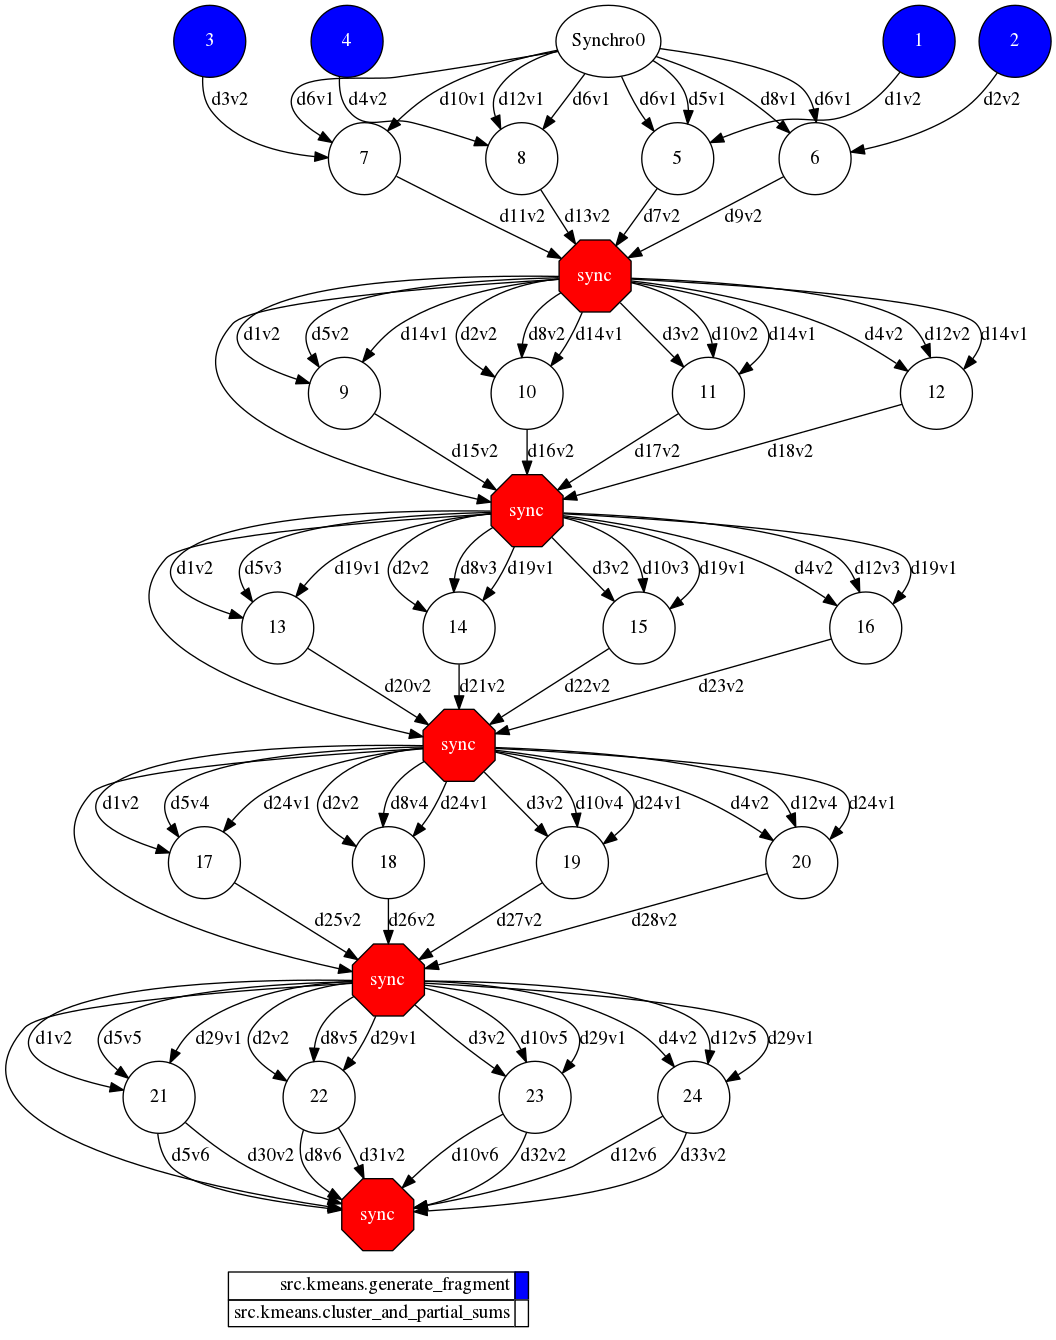
\includegraphics[scale = 0.3]{figures/kmeans_storage_dep_graph.png}
\caption{Dependency graph of a 6-iteration K-Means execution with $4$ point fragments.}
\label{fig:kmeans_storage_dep_graph}
\end{figure}

\begin{figure}[ht!]
\centering
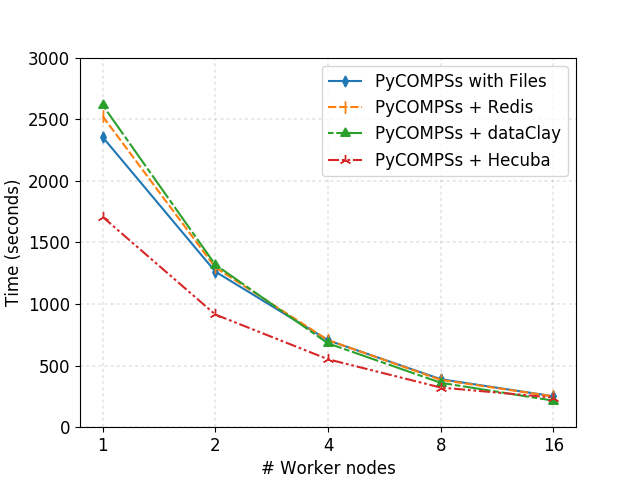
\includegraphics[scale = 0.5]{figures/storage/kmeans_strong.png}
\caption{Strong scaling graph of our various storage implementations}
\label{fig:kmeans_strong_redis}
\end{figure}


\begin{figure}[ht!]
\centering
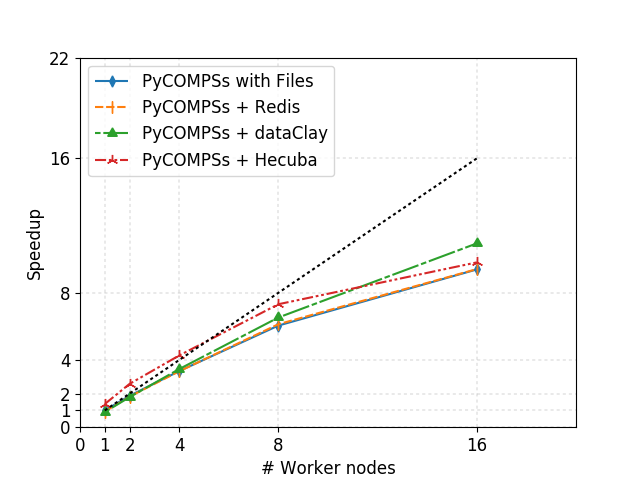
\includegraphics[scale = 0.5]{figures/storage/kmeans_strong_speedup.png}
\caption{Strong scaling speedup graph of our various storage implementations}
\label{fig:kmeans_strong_speedup_redis}
\end{figure}


\begin{figure}[ht!]
\centering
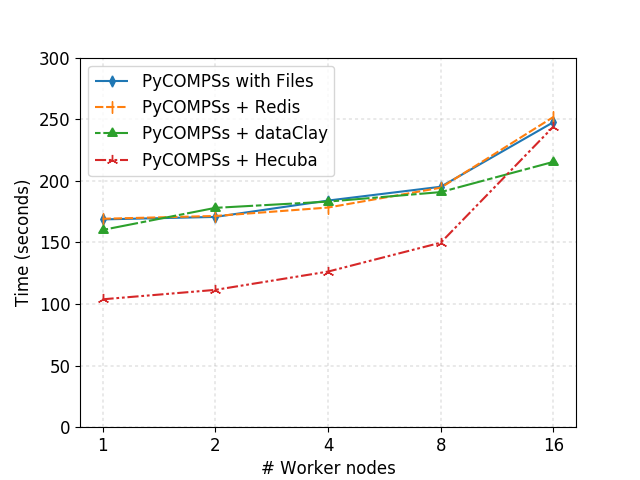
\includegraphics[scale = 0.5]{figures/storage/kmeans_weak.png}
\caption{Weak scaling graph of our various storage implementations}
\label{fig:kmeans_weak_redis}
\end{figure}


\begin{figure}[ht!]
\centering
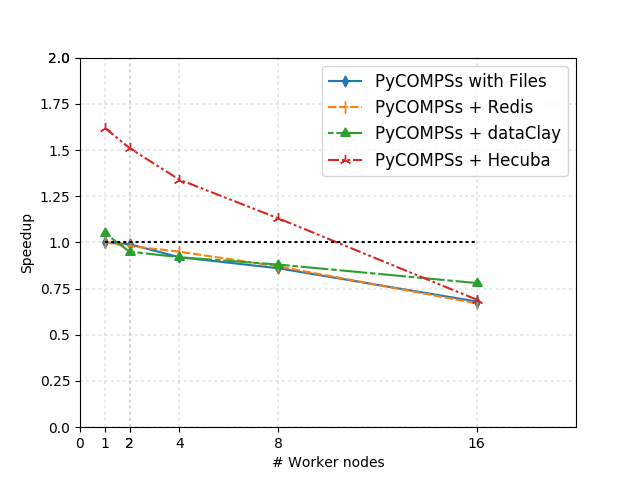
\includegraphics[scale = 0.5]{figures/storage/kmeans_weak_speedup.png}
\caption{Weak scaling speedup graph of our various storage implementations}
\label{fig:kmeans_weak_speedup_redis}
\end{figure}

As we can see, our storage implementation does not improve the overall performance of this application. However, as we can see in figure \ref{fig:kmeans_transfer_trace}, this applications has little to no heavy transfers, only at the beggining, so these results are more or less expected.


%TODO: GET THE KMEANS TRACE

\subsubsection{Matrix Multiplication}
\label{subsubsec:matmul_redis}
The matrix multiplication is a very common algorithm and it is usually the preferred example of what an embarrassingly parallel application is (i.e: a parallel application with no dependencies). Its distributed version is also interesting but due to other property: the enormous amount of required data transfers. Let's take a look to the following code:

\inputminted{python}{snippets/matmul_python.py}

This code can be parallelized in any of the three loops. The only special requirement is to make sure 



As we can see in figures \ref{fig:matmul_strong_redis} and \ref{fig:matmul_strong_speedup_redis} the Matrix Multiplication gets a huge benefit from our storage systems.

\begin{figure}
\centering
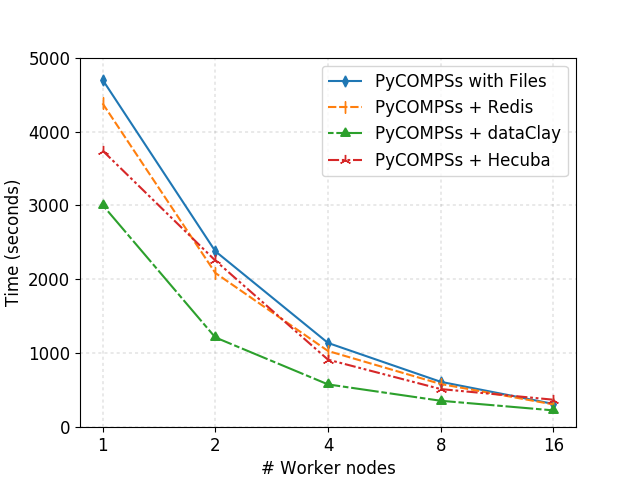
\includegraphics[scale = 0.5]{figures/storage/matmul.png}
\caption{Strong scaling graph of our various storage implementations}
\label{fig:matmul_strong_redis}
\end{figure}



\begin{figure}
\centering
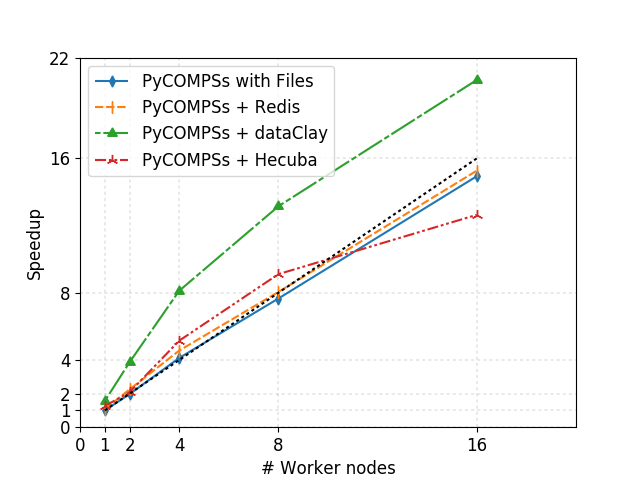
\includegraphics[scale = 0.5]{figures/storage/matmul_speedup.png}
\caption{Strong scaling speedup graph of our various storage implementations}
\label{fig:matmul_strong_speedup_redis}
\end{figure}

